%\documentclass[a4paper,10pt]{article}
\documentclass{article}

\title{Physics Investigation. Determining the Goldilock Zones for 8 stars of different types. }
\date{}
\author{}
\usepackage{url}
\usepackage{setspace}
\usepackage{hyperref}
\usepackage{graphicx}
\usepackage{amsmath}
\usepackage{listings}
\usepackage{color}
\usepackage{multicol}
\usepackage{caption}
\usepackage{subcaption}

\begin{document}
% --------------- COVER PAGE STARTS HERE ---------------
\maketitle
%\begin{center}
%  Physics Investigation.\\
%\end{center}


\begin{figure}
  \begin{flushleft}
    Session: May 2018\\
    \end{flushleft}
  \end{figure}

%\newpage


\tableofcontents
\newpage

% ---------------  QUOTE STARTS HERE   ---------------
%\newpage
\begin{center}
  "If we stay on Earth forever, there will be some eventual extinction event." 
\end{center}
\begin{flushright}
  -Elon Musk \cite{musk}
\end{flushright}
% ---------------    QUOTE ENDS HERE   ---------------


\begin{abstract}
  This physics Investigation is called ``Determining the Goldilocks Zone for 8 stars of different types''.
  During this investigation, I will pick 8 stars of different types: White Dwarfs, Red Giants, Main-Sequence Stars and Red Dwarfs.
  I will research the stars in terms of luminosty, radius and the length of Goldilock Zones, more known as Circumferential Habitable Zones.\\
  
  During this research, I will investigate different properties and charasteristics of a star to determine its habitability.
  At the end of the research, we will understand which star types are more preferrable for life.\\
  
  For the sake of demonstration, I have written several programs and simulations to support my investigation. All of the source code is available on my Github page in the ``pyhyg'' repository. \cite{github}\\
  
\end{abstract}



%\newpage
%\pagenumbering{arabic}
%\doublespacing
%\onehalfspacing
% --------------- COVER PAGE ENDS HERE ---------------


% -------------    PICTURE STARTS HERE   ---------------
%\begin{center}
%\begin{figure}[b!]
  %\centering
%  \begin{center}
%    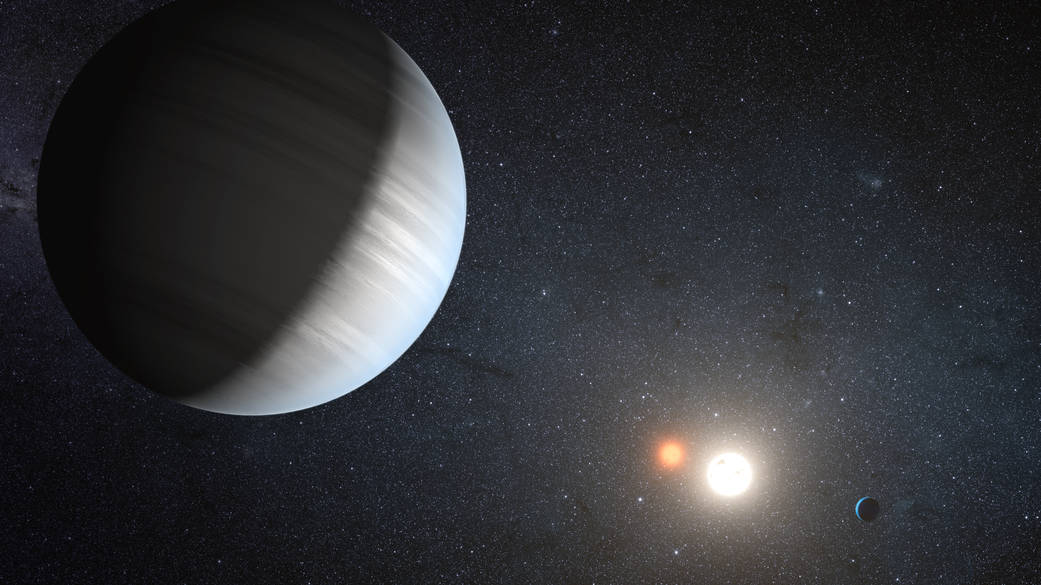
\includegraphics[width=0.8\textwidth]{kepler.jpg}
%    \caption{Sharing the Light of Two Suns~\cite{kepler}}
%  \end{center}
  
%\end{figure}
%\end{center}
% -------------    PICTURE ENDS HERE   ---------------
%\doublespacing


%\newpage

\section{Inroduction}

Soon, our Mother-Star, Sun will make the poles of Earth a tropical paradise and later on destroy all the life on Earth. Approximately in 5.4 billion years, the critical amount of hydrogen in Sun's core will be depleted. In that event, because of lack of hydrogen, Sun will start collapsing under its own weight. The delicate balance between fusion energy and the gravitational pull has fallen.\\

This catastrophic event forces the core of our Star to contract and therefore, to start fusion of Helium and more heavy elements. This will stop the active contraction of the star but in this event, Sun will burst a colossal amount of energy into outer layers, thus increasing in size so much, that out star will ``consume'' Mercury and Venus, scientists are not sure about Earth. We can be sure in one fact -  by that time, all the life on Earth will be ceased. Indeed, life will cease to exist way before the Sun's Red Giant phase.\\

Around in 1.1 billion years, Sun's luminosity will increase by about 10\%. It seems not that much, however, this increase in luminosity will cause a very big shift in Sun's Goldilock zone length. The more active greenhouse effect will take place on Earth, transforming our home planet into a hot, dry and unhabitable planet that Venus is right now.~\cite{sun}\\

As the means of humanity's future survival, we will be forced to leave our planet Earth and find a new planet, new home that maybe can recall our Earth. In order to do that, we should know which planets are habitable and which are not. I will take 8 stars of different types to figure out, what types of stars can host life.\\

\section{Investigation data}

\subsection{Research question}

My phsyics investgation is aimed at finding the best odds of living near different types of stars, more differentiated by their spectral type. These include: White Dwarfs, Red Giants, Red Dwarfs, and Main-Sequence Stars.\\

\textbf{The research question is}

\textit{What is the relationship between the conditions of existence of life in the Goldilock Zone versus star's spectra and type }

\subsection{Hypothesis}

Today, life on Earth is the only known habited planet. We have no information or confirmation about the existence of other life forms and species on other extraterrestial objects. Earth rotates its home star - Sun, which is a typical member of Main-Sequence stars.\\

\textbf{My hypothesis is}

  \textit{The most favorable conditions for life formations are near the members of Main-Sequence stars.}

  \subsection{Outside of the syllabus}

  The topic and the concepts that I am exploring are mostly outside the curriculum of Physics: Option D Astrophysics. The topic of Circumferential Habitable Zones of stars are not explored or mentioned in the guides. During the investigation, Luminosity and Apparrent Brightness formulas from the Physics Guide will be used. 

  
\section{Initial set of data and choices}

  \subsection{Database}
  \label{database}
  The HYG Database \cite{hyg} will be used for extraction and parsing of astronomical data. The database contains more than 120,000 stars and it can provide me with the needed data, as the apparent visual magnitudes of stars. Further information and details about the database's entries can be found in in the references.\\  
  
%  \newpage
  \subsection{Stars}
  
  Now, we need to choose our 8 stars. For the sake of demonstration and visualization, I wrote a small program in Python that takes the values from the database from part \ref{database} and plots Hertzprung-Russel Diagram. Note that instead of luminosity and temperature, values of absolute visual magnitutes and color indexes are used.\\
  
  I will take 8 stars of 4 different types, so 2 stars of each type. In the next table, Red Dwarfs, Main-Sequence stars, Red Giants, White Dwarfs are presented, respectively. Table \ref{stars} demonstrates 8 stars that I chose for research.\\
  
  \begin{table}[h!]
    \begin{center}
      \caption{Chosen 8 stars for the investigation.}
      \begin{tabular}{l | l | l | l}
        \textbf{GlieseID} & \textbf{Star name} & \textbf{Type} & \textbf{Spectra}\\
        \hline
        551  & Proxima Centauri & Red Dwarf     & M5Ve\\
        623  & Gliese 623       & Red Dwarf     & M3\\
        482A & 29Gam Vir        & Main-Sequence & FOV+...\\
        231  & Alp Men          & Main-Sequence & G5V\\
        286  & Pollux           & Red Giant     & K0IIIvar\\
        841  & HD 208527        & Red Giant     & M0\\
        35   & Van Maan         & White Dwarf   & DG\\
        440  & LP 145-141       & White Dwarf   & DC:\\
      \end{tabular}
      \label{stars}
    \end{center}
  \end{table}
  
  The results of the program are demonstrated below. Figure \ref{full} is the result of the program, when 4715 random stars from our database are plotted. We can clearly see that it is indeed the HR diagram with the necessary zones. On the other hand, Figure \ref{str} shows the Hertzprung-Russel Diagram only with out 8 stars, which were mentioned in Table \ref{stars}.\\

  On the Figure \ref{str}, we see how each 2 stars are located in different sections of the HR Diagram, therefore proving that our stars are from different types of stars. The source code and example output of all the programs and simulations written and used for this investigation are available on my Github page.\cite{github}\\
  
  \begin{figure}[h]
    \centering
    \begin{minipage}[b]{0.45\textwidth}
      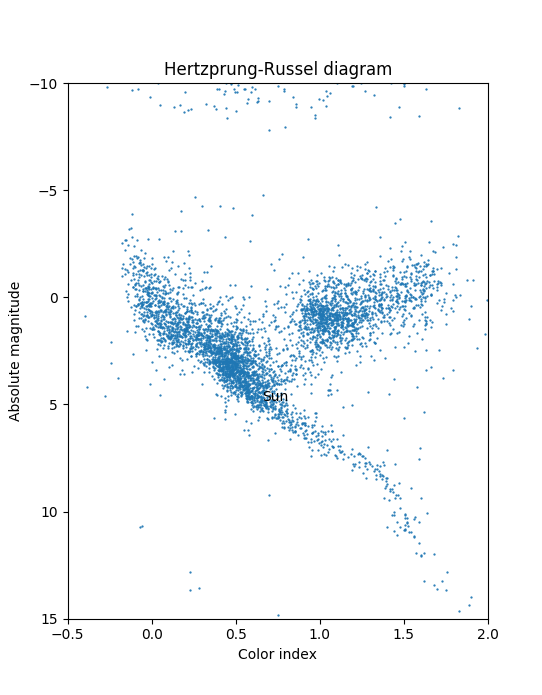
\includegraphics[width=\textwidth]{full.png}
      \caption{Hertzprung-Russel Diagram with 4715 stars.}
      \label{full}
    \end{minipage}
    \hfill
    \begin{minipage}[b]{0.45\textwidth}
      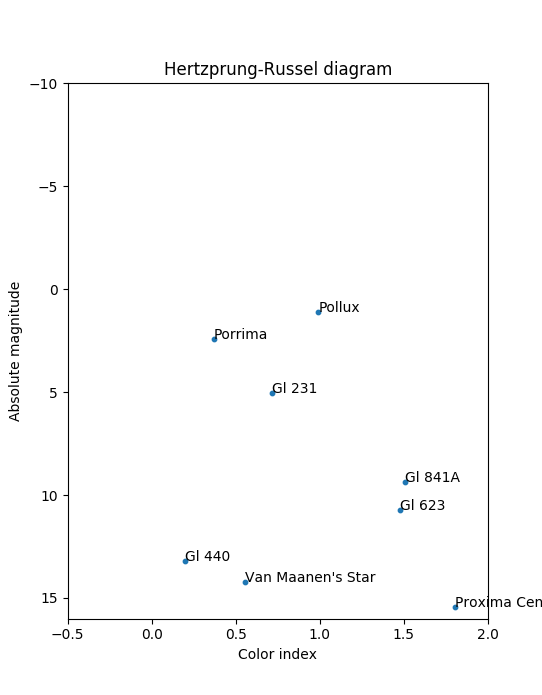
\includegraphics[width=\textwidth]{stretch.png}
      \caption{Hertzprung-Russel Diagram with our 8 stars.}
      \label{str}
    \end{minipage}
  \end{figure}
  
  
  %\newpage
%  \onehalfspacing
  \section{Variables list}
  
  \subsection{Dependent variables}
  
  \begin{itemize}
    
  \item Absolute Visual Magnitude of a star, $M_V$ ($unit$)
    
    \begin{itemize}
      
    \item This is Apparent Visual Magnitude of a star that is seen from a distance of 10 parsecs or 32.6 light years
      
    \end{itemize}
    
  \item Inner Edge of Goldilock Zone of a star, $r_i$ ($AU$) 
    
  \item Outer Edge of Goldilock Zone of a star, $r_o$ ($AU$)
    
  \item Bolometric Magnitude, $M_{bol}$ ($unit$)
    
  \item Apparent Brightness, $b$ ($W m^{-2}$)

  \item Luminosity of a star, $L_*$ ($W$)
    
  \item Absolute Luminosity, $L_{star}$ ($W$)

    \begin{itemize}
      
    \item This is the ratio of the luminosty of a star to solar luminosity, $\frac{L_*}{L_{\odot}}$
      
    \end{itemize}
    
  \end{itemize}
  
  
  \subsection{Independent variables}
  
  \begin{itemize}
    
  \item Astronomical distance to a star, $d$ ($pc$)
    
  \item Apparent Visual Magnutuse of a star, $M$ ($unit$ *from database)
    
  \item Bolometric Correction, $BC$ ($unit$ *from database)
    
    \begin{itemize}
      
    \item This is a correction made to the star's absolute visual magnitude in order to convert its
      visible magnitude into bolometric magnitude.
      
    \end{itemize}    
    
  \end{itemize}
  
  \subsection{Controlled variables}
  
  \begin{itemize}
    
  \item Stefan-Boltzmann constant, $\delta$ ($5.67 \times 10^{-8} W m^{-2} K^{-4}$)
    
  \item Solar Luminosity, $L_{\odot}$ ($3.828 \times 10^{26}W$)
    
  \item Astronomical Unit, $AU$ ($150 \times 10^{9}m$)

  \item Solar Bolometric Magnitude, $M_{bol, \odot}$ ($+4.74$)
    
  \end{itemize}
  
  
%  \doublespacing
%  \newpage
  
  
  \section{Main calculations}
  
  As now, I have discussed and presented all the initial data, now is the time to start the calculations and physical research. Please not that all the calculation will not be represented in a classical 3 significant figures way. Because astrophysics deals with very large or very small values, there is a need of using values with high preciseness. \\
  
  Firstly, we should know the distance and Apparent Visual Magnitude of our stars. Table \ref{data} shows the data that was pulled from the database.
  
  \begin{table}[h!]
    \begin{center}
      \caption{Initial data of the stars}
      \begin{tabular}{c | c | c}
        \textbf{GlieseID} & \textbf{Distance (pc)} & \textbf{Apparent Magnitude} \\
        \hline
        551  & 1.2959  & 11.010\\
        623  & 8.0567  & 10.270\\
        482A & 11.6850 & 2.740\\
        231  & 10.1978 & 5.080\\
        286  & 10.3584 & 1.160\\
        841  & 15.9719 & 10.360\\
        35   & 4.2626  & 12.370\\
        440  & 4.6081  & 11.500\\
      \end{tabular}
      \label{data}
    \end{center}
  \end{table}
  
  \subsection{Absolute Visual Magnitude}

  Secondly, Apparent Visual Magnitudes and Absolute Visual Magnitudes are practically the same but with 1 key difference. If Apparent Magnitude shows how bright the star is from point of view of Earth, Abolsute Magnitude shows us how bright the star is in comparison will all other stars in the universe. This is important, because we need a unified metrics of stars, which are put on ``equal'' conditions. I found a formula that uses Apparent Visual Magnitude and the distance to a start to calculate the Absolute Visual Magnitude.
  
  \begin{equation}
    {100}^{\frac{M-M_V}{5}} = {(\frac{d}{10pc})}^2\\
  \end{equation}

  After some rearrangments and logarithmic manipulations, we get:

  \begin{equation}
    M_V = M - 5(\log_{10}{(d_{pc})}-1)\\
    \end{equation}
    
  Now, with this knowledge, we can find precise and accurate values of our stars' Absolute Visual Magnitudes. All the calculations will
  be performed by using Wolfram Alpha Calculator.\\
  
\begin{table}[h!]
    \begin{center}
      \caption{Calculations of stars' Absolute Magnitudes}
      \begin{tabular}{c | c | c}
        \textbf{GlieseID} & \textbf{Absolute Magnitude} & \textbf{Abs. Magnitude (4sf)}\\
        \hline
        551  & 15.447142550675103 & 15.447\\
        623  & 10.739214037414767 & 10.739\\
        482A & 2.401856416358772  & 2.402\\
        231  & 5.037467548500953  & 5.037\\
        286  & 1.0835366113876055 & 1.084\\
        841  & 9.343217087925737  & 9.343\\
        35   & 14.221627096960558 & 14.222\\
        440  & 13.182390524468321 & 13.182\\
        
      \end{tabular}
      \label{avm}
    \end{center}
  \end{table}
  
We have found the values of our first variables in the problem, we may proceed.

\subsection{Bolometric Correction and Magnitude}
\label{bcm}
We have found absolute magnitudes of our stars. The next step we need to take is finding the Bolometric Magnitude of our stars. Bolometric magnitude is the absolute magnitude of a star that takes into account electromagentic radiation of a star with all its wavelenegths. It is defined based on the luminosity of a star. Further on, it will help us later to find the ration of star's luminosity to a solar luminosity.\\

Firstly, Table \ref{bc} demonstrates how the values of Bolometric Corrections are assigned to individual spectral types. I will use the extended version of the original Kaler table\cite{kaler}. Because we have 8 stars with different spectral types, we need to use more accurate data for the results to be exact. Bolometric correction is the correction that has been made to Absolute Magnitudes of stars in order to convert its visual magnitude to Bolometric Magnitude.\cite{bc}\\
  
  \begin{table}[h!]
    \begin{center}
      \centering
      \caption{The relationship between Bolometric Correction and star's spectral type.}
      \begin{tabular}{c | c}
        \textbf{Spectral Type} & \textbf{Bolometric Correction} \\
        \hline
        O5 & -4.0 \\
        B0 & -2.8 \\
        B5 & -1.5 \\
        A0 & -0.4 \\
        A5 & -0.12\\
        F0 & -0.06\\
        F5 & 0.00 \\
        G0 & -0.03\\
        G5 & -0.07\\
        K0 & -0.2 \\
        K5 & -0.6 \\
        M0 & -1.2 \\
        M5 & -2.3 \\
      \end{tabular}
      \label{bc}
    \end{center}
  \end{table}

  Secondly, after applying the data from Table \ref{bc}, we are able to assign Bolometric Correction values to our stars. If some stars have spectral type nor with 0 nor with 5, I will average the Bolometric Correction. For example, if a star has spectral type ``K2.5'', I will take the average between K0 and K5 and later assign that value. Table \ref{bcv} demonstrates the distribution of Bolometric Correction values on the stars.\\


\begin{table}[h]
    \begin{center}
      \caption{Stars' Bolometric Correction values}
      \begin{tabular}{c | c | c}
        \textbf{GlieseID} & \textbf{Spectral Type} & \textbf{Bolometric Correction}\\
        \hline
        551  & M5Ve     & -2.3\\
        623  & M3       & -1.86\\
        482A & FOV+...  & -0.06\\
        231  & G5V      & -0.07\\
        286  & K0IIIvar & -0.2\\
        841  & M0       & -1.2\\
        35   & DG       & 0\\
        440  & DC:      & 0\\
      \end{tabular}
      \label{bcv}
    \end{center}
  \end{table}
  
  Thirdly, as because the Bolometric Correction is the correction of Absolute Visual Magnitude to Bolometric Visual Magnitude, this means that the formula for Bolometric Correction of a star will look like this:

  \begin{equation}
    BC = M_{bol} - M_V\\
    \end{equation}

  After some simple rearrangements, we can express the Bolometric Magntiude in terms of already known variables

  \begin{equation}
    M_{bol} = BC + M_V\\
    \end{equation}

  With the values of Bolometric Correction from Table \ref{bcv} we can find the values of Bolometric Magntudes for our stars. All the calcualtions below are performed by using Wolfram Alpha Calculator. The result of the calculation are presented in Table \ref{mbol}\\

\begin{table}[h]
    \begin{center}
      \caption{Stars' Bolometric Magnitude values}
      \begin{tabular}{c | c}
        \textbf{GlieseID} & \textbf{Bolometric Magnitude}\\
        \hline
        551  & 13.147\\
        623  & 8.879\\
        482A & 2.342\\
        231  & 4.967\\
        286  & 0.884\\
        841  & 8.143\\
        35   & 14.222\\
        440  & 13.182\\
      \end{tabular}
      \label{mbol}
    \end{center}
  \end{table}
    
\subsection{Lumonosity}

\subsubsection{Information}

Luminosity is best desribed as the amount of power radiated by a Black Body like object. The basic formula from out syllabus is the following

\begin{equation}
  L = \delta AT^4\\
  \end{equation}

\subsubsection{Stars' Luminosities}

We will find the lumonisities of ours stars in terms of solar luminosity ($L_{\odot}$). In order to do that, I will use the formula of relationship of Bolometric Magnitude and the ratio of lumonisties, where $M_{bol, *}$ and $L_*$ are Bolometric Magnitude and Luminosity of a star, respectively.

\begin{equation}
  M_{bol, *} - M_{bol, \odot} = -2.5 \log{10}{(\frac{L_*}{L_{\odot}})}\\
  \end{equation}

After some rearrangements, we can express the formula in the way that we can find the Luminosity of a star in relationship to Solar Luminosity.

\begin{equation}
  L = \frac{L_*}{L_{\odot}} = 10^{\frac{M_{bol, *} - M_{bol, \odot}} {2.5}} = 10^{0.4(M_{bol, *} - M_{bol, \odot})}\\
  \end{equation}

With the data gained from \ref{bcm}, we can find the lumonisities of our 8 stars. I will use Wolfram Alpha as a calculator. The results are presented in Table \ref{lum}    \\

\begin{table}[h]
    \begin{center}
      \caption{Stars' Absolute Luminosity values}
      \begin{tabular}{c | c | c}
        \textbf{GlieseID} & \textbf{$L_{star}$} & \textbf{$L_{star}$} (9sf)\\
        \hline
        551  & 0.00043365362363341085 & 0.00043365 \\
        623  & 0.02209603682544578    & 0.02209604 \\
        482A & 9.104527949318182      & 9.10452795 \\
        231  & 0.8109852969785725     & 0.8109853 \\
        286  & 34.880713131600245     & 34.88071313 \\
        841  & 0.04352243294403225    & 0.04352243 \\
        35   & 0.000161194107212134   & 0.00016119 \\
        440  & 0.000419801310713262   & 0.0004198 \\
      \end{tabular}
      \label{lum}
    \end{center}
  \end{table}

Please note that the values that I have calculated might differ from official ones. This innacuracy can happen because of innaccuracies in formulas. As I use the simplified and generalized versions of formulas, instead of closed or non-published more accurate formulas. 

\subsection{Circumferential Habitable Zones}

For this investigation we will find the lengths of Goldilock Zones of our stars. According to an article by Tom. E. Morris \cite{habz}, the formulas of the inner and outer edges of Circumstellar Habitable are the following

\begin{equation}
  r_i = \sqrt{\frac{L_{star}}{1.1}}\\
  \end{equation}

\begin{equation}
  r_o = \sqrt{\frac{L_{star}}{0.53}}\\
  \end{equation}

Now, we are able to find the answer. All the calculations are performed by Wolfram Alpha. All the values are calculated in terms of Astronomical Unit, which is the distance from Sun to Earth. It is done in this way, so it is easier to understand the ranges in comparison with out Solar System. The results are presented in Table \ref{chz}.


\begin{table}[h]
    \begin{center}
      \caption{Stars' Absolute Luminosity values}
      \begin{tabular}{c | c | c | c}
        \textbf{GlieseID} & \textbf{$r_i$} \textbf{($AU$)} & \textbf{$r_o$} \textbf{($AU$)} & \textbf{$r_o - r_i$} \textbf{($AU$)}\\
        \hline
        551 & 0.02 & 0.03 & 0.01\\
        623 & 0.14 & 0.2 & 0.06\\
        482A & 2.88 & 4.14 & 1.27\\
        231 & 0.86 & 1.24 & 0.38\\
        286 & 5.63 & 8.11 & 2.48\\
        841 & 0.2 & 0.29 & 0.09\\
        35 & 0.01 & 0.02 & 0.01\\
        440 & 0.02 & 0.03 & 0.01\\
      \end{tabular}
      \label{chz}
    \end{center}
  \end{table}

We have found the Goldilock Zones of our 8 stars.

\section{Further Calculations}

I thought that 8 stars is not quite enough to judge the hospitability of different star types. I decided to write a program that will take into the account around 120,000 stars and find the length of CHZ.\\

Before introducing the program, I should find the general formula for finding the range of CHZ. Taking into the account all previous section, we can derive this nice formula

\begin{equation}
  r_o - r_i = \sqrt{\frac{10^{0.4(M_{BC + M - 5(\log_{10}{(d_{pc})}-1)} - M_{bol, \odot})}}{0.53}} - \sqrt{\frac{10^{0.4(M_{BC + M - 5(\log_{10}{(d_{pc})}-1)} - M_{bol, \odot})}}{1.1}}\\
  \end{equation}










% --------------- REFERENCES START HERE ------------------
\newpage
\bibliographystyle{ieeetr}
\bibliography{main}
% --------------- REFERENCES  END  HERE ------------------
  \end{document}
